% !TeX spellcheck = en_US
% !TeX encoding = UTF-8
% !TeX root = ../document.tex

\chapter{Optimization of the Algorithm}
In this chapter, the optimal value for the Quickscan parameter \paramregions is determined. This value highly impacts performance and statistical accuracy. Possible approaches for a trade-off between speed and quality will be proposed.

\section{Metrics}
The optimization is performed in regard of the goals described in chapter \ref{ch:quickkscan_motivation}: Statistical performance and required computation time. The comparison reference in both cases is the execution of the scanning algorithm without Quickscan. This scenario is called \emph{full scan} here.

\subsection{Statistical Sensitivity}
The statistical sensitivity is measured as deviation of \ptilde. To calculate this deviation, the trial scanning run is compared to a reference run with the same settings. Since the \ptilde~value is only evaluated for distributions with a RoI \p~value of $< \num{0.3}$, the reference as well as the sample run only contain \ptilde~values for a subset of event classes (usually about half).

For each event class, the \ptilde~value of the reference run is compared to the corresponding \ptilde~value of the trial run:
\begin{equation}
	\sigmarel = \frac{\Delta \ptilde}{\ptilde_\mathrm{reference}} = \frac{\ptilde_\mathrm{sample} - \ptilde_\mathrm{reference}}{\ptilde_\mathrm{reference}}
\end{equation}
Usually, a full scan is used for $\ptilde_\mathrm{reference}$, while a run with the Quickscan yields $\ptilde_\mathrm{sample}$.

\begin{figure}
	\centering
	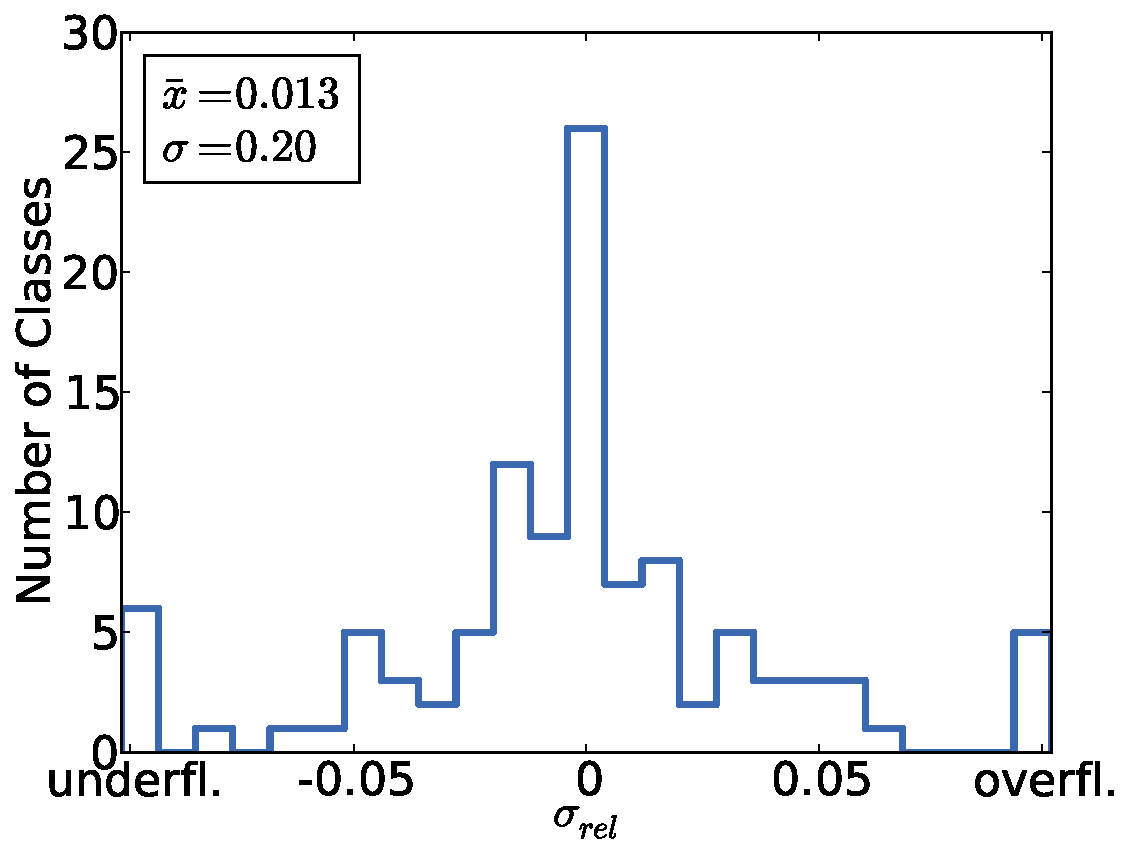
\includegraphics[width=0.6\linewidth]{delta_p_tilde_random_deviation}
	\caption{Random deviation of \sigmarel. Obtained by comparing two sets of scan results without the Quickscan algorithm. The distribution spread of $\order{\SI{5}{\percent}}$ originates in the random means of the pseudo experiments. This also demonstrates that only a few classes show no deviation at all.}
	\label{fig:delta_p_tilde_random_deviation}
\end{figure}

Figure \ref{fig:delta_p_tilde_random_deviation} shows a comparison between two separate full scans. Here, one full scan is used as reference, the other one as sample. The visible deviation of \sigmarel is caused by the random dicing of pseudo experiments while calculating \ptilde (see section \ref{sec:music_ptilde}). The conclusion of this illustration is that dicing the pseudo-experiments introduces a statistical uncertainty of $\order{\SI{5}{\percent}}$ on the \ptilde~value. This value will act as guideline for the Quickscan parameter choice.

\subsection{Computation Time}
There are various approaches to comparing the computation costs of computer programs: A commonly used option is to count the number of CPU cycles that a program has used. This method allows for comparisons with a high resolution, but this "pure" CPU time does not represent the time spent on a real-world application. Additionally, it is difficult to implement, especially in an environment like the MUSiC scanning algorithm because of multitasking and the usage of various technologies (Python and C++). 

The alternative technique used in this work is \emph{wall-clock time}. The measurement of wall-clock time is performed by acquiring a timestamp before and after the execution of the program. The elapsed time is the difference between those two timestamps. The results of such measurement can be directly transfered to the real-world application because it is performed in the same environment as an execution on a user machine.

This method introduces the following systematic uncertainties:
\begin{my_list}
	\item CPU usage by other processes: The measurement is performed on a system shared by multiple users. The operating system distributes the available CPU resources between the user processes. Thus, the benchmarked program runs significantly slower if other computation intensive processes are present. In order to suppress this effect, it is ensured that at the time of the measurement, the machine is not occupied by other users. The influence can be lowered this way, from $\order{\num{e-1}}$ to $\order{\num{e-2}}$.
	\item IO throughput: The files required by the scanning algorithm are stored on shared network drives. Similarly to the CPU usage, the behavior of other users influences the measured wall-time (also $\order{\num{e-2}}$).
	\item Static overhead: The measurement includes operations that are not being optimized and contribute a constant amount of time. Examples are reading and parsing of parameters and configuration, creating and destroying multitasking worker processes and writing output files. This takes up $\order{\num{e-2}}$ of the total time but is expected to be almost constant.
	\item Timestamp resolution: Although the operating system's internal clock has a high resolution, the results are only written to file with a resolution of \SI{1}{\second}. In comparison to the other uncertainties, this is negligible ($\order{\num{e-4}}$). 
	\item Time adjustments: The time on the computing host is managed by the Network Time Protocol (NTP). It ensures time synchronization inside the datacenter. If the NTP daemon notices that either the time of the host has shifted or if leap seconds are introduced, the host time is adjusted. This has an effect on the acquired timestamps but is highly negligible in this scenario ($\order{\num{e-6}}$).
\end{my_list}

The computation improvement is quantified by the ratio between the wall-clock time measurement of the full scan and the Quickscan algorithm:
\begin{equation}
	\textrm{speedup} = \frac{T_{\textrm{full}}}{T_{\textrm{quickscan}}} \geq 1 
\end{equation}


\section{Optimization Environment}
The optimization is performed in \num{60} processes on a 64-core MUSiC host, whose specifications are listed in table \ref{tbl:music_machine}. The wall-time is measured for the entire execution of the main scanning script (\texttt{MISMaster.py}).

\begin{table}
	\centering
	\begin{tabular}{ l l }
		\toprule
		processors & AMD Opteron Processor 6272 \\
		clock speed & \SI{2.1}{\giga\hertz} \\
		cores per CPU & 8 logical (4 physical) \\
		total number of cores & 64 \\
		memory & $\approx \SI{250}{\giga\byte}$ \\
		\midrule
		operating system & Linux \\
		kernel version & 2.6.32-504.16.2.el6.x86\_64 \\
		distribution & Scientific Linux release 6.5 (Carbon) \\
		\midrule
		CMSSW version & 5.3.14 \\
		GCC version & 4.7.2 \\
		Python version & 2.6.4 \\
		\bottomrule 
	\end{tabular}
	\caption{Specification of the 64-core machine on which the computation measurement is performed.}
	\label{tbl:music_machine}
\end{table}

As shown earlier, \sigmarel deviates by about \SI{5}{\percent} through random dicing. The optimization should occur isolated from this deviation. 

The first measure against random influences is to seed the pseudo random number generator (PRNG) with a fixed value. 
Additional non-determinism is introduced by the parallelization implementation. An optimization called \emph{hit-threshold} allows the Quickscan to stop generating pseudo-experiments once the \ptilde value is determined to a sufficient precision. Not all parallelized workers can be terminated in a deterministic sequence, the actual order depends on uncontrollable external factors. Subsequently, the PRNG state is not deterministic. To counteract this effect, the hit-threshold method is turned off.

Because of degraded overall performance, only \num{e3} pseudo-experiments are generated and evaluated, as opposed to up to \num{e5} in normal operation mode.

Determinism of this configuration is evaluated by comparing the results of two full scans. The comparison yields absolutely no deviation in \sigmarel.

\section{Execution}
The optimization run is performed on a subset of data from 2012 taken at ${\sqrt{s} = \SI{8}{\TeV}}$. Only the \sumpT distribution of all exclusive event classes is regarded. Additionally, for a given combination of leptons, all events containing at least \num{2} jets are summarized in one event class \eventclass{... + 2jet + Njet}.
In order to save time, classes with a data \p~value above \num{0.3} are excluded from the \ptilde calculation and thus excluded from the Quickscan, which is only applied on pseudo-experiments. This reduces the number of regarded classes from \num{214} to \num{108}. The full settings are listed in the appendix, in the left column of table \ref{tbl:music_configuration}.

For each parameter value, the scanning step is executed \num{5} times using \num{60} processes each. The raw measurement results can be found in tables \ref{tbl:deltaptilde_results} and \ref{tbl:timing_results} in the appendix. Figure \ref{fig:parametersweep} illustrates these results. The horizontal axis shows the parameter value for \paramregions, the vertical axes show the runtime speedup and the number of classes where the Quickscan \ptilde~value does not deviate from the full scan \ptilde within its uncertainty. The vertical error bars on the speedup measurement indicate the uncertainty of the mean speedup value and have been obtained by calculating the sample error of the \num{5} trial results. As expected, this deviation is up to $\order{\num{e-1}}$ due to the uncertainties discussed above.

\begin{figure}
	\centering
	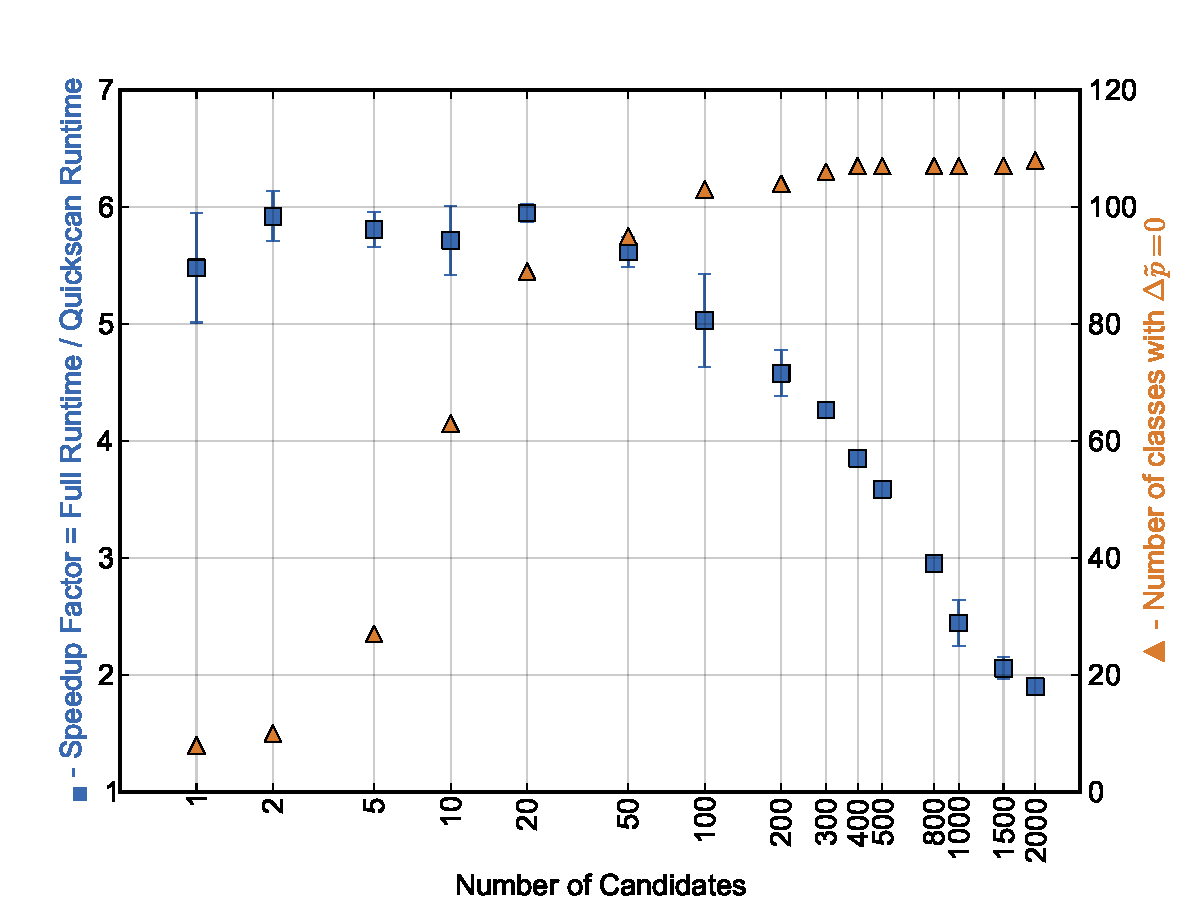
\includegraphics{parametersweep}
	\caption{Combined results of the runtime and $\Delta \ptilde$ measurement for varying numbers of Quickscan RoI candidates. The error bars on the speedup measurement indicate the uncertainty $\sigma_{\overline T} = \sigma_T / \sqrt{N}$ on the mean $\overline T$ during the \num{5} trial runs. As expected with a deterministic run, there is no uncertainty of $\Delta \ptilde$.}
	\label{fig:parametersweep}
\end{figure}

\section{Analysis}
The results match the expectations: a larger number of candidates raises the chances of including the "true" RoI inside the number of candidates. This improves the accuracy of \ptilde, such that more classes show no deviation ($\Delta \ptilde = 0$, $\sigma_\mathrm{rel} = \num{0}$). Thus, the number of classes without deviation converges to the total number of classes (\num{108}). In the same limit, the speedup value tends towards \num{1}, which indicates that the Quickscan takes the same amount of time as the full scan in that case.

Figure \ref{fig:parametersweep} shows that even for \num{1500} candidates, one class has $\Delta \ptilde \neq 0$. The affected event class is \eventclass{3e}, which has a full scan $\ptilde = \num{0.735}$ and shows a deviation of $\Delta \ptilde= \num{-0.001}$. Since this difference is insignificant, it is not further discussed here.

To obtain a recommendation value for \paramregions, the $\Delta \ptilde$ result should be compared with figure \ref{fig:delta_p_tilde_random_deviation}, which showed that the spread induced by random dicing only preserves \ptilde for a few classes. Taking \num{5} candidates, the spread induced by the Quickscan has a similar magnitude. Figure \ref{fig:delta_p_tilde_examples} shows that for $\paramregions > \num{100}$ the width of the distribution is negligible. 

Note that while the \p~value of data $\p_\mathrm{data}$ is unaffected by the Quickscan, a pseudo experiment's \p~value obtained with the Quickscan is larger or equal to the \p~value which would have been obtained by the full scan. The full scan calculates the \p~value for all connected regions, while the Quickscan calculates the \p~value only for its candidate regions. Thus, for the Quickscan less pseudo experiments show a more significant deviation than $\p_\mathrm{data}$, resulting in a smaller (or equal) overall \ptilde~value. Because of that, the $\sigma_\mathrm{rel}$ distribution of Quickscan results is asymmetric.

\begin{figure}
	\centering
	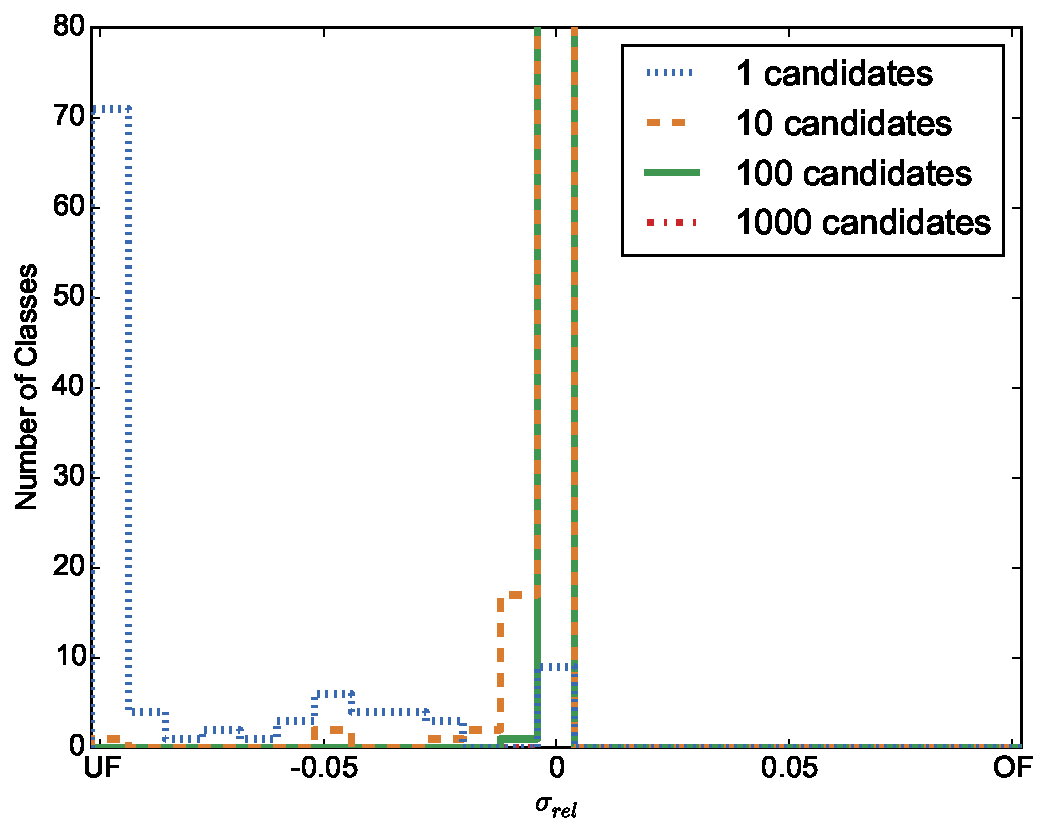
\includegraphics{delta_p_tilde_examples}
	\caption{Deviation of \sigmarel due to the Quickscan algorithm. When taking more than \num{10} candidates, the spread is less than \SI{1}{\percent} and can be neglected compared to the other random influences.}
	\label{fig:delta_p_tilde_examples}
\end{figure}


\section{Optimization Conclusion}
Concluding, this analysis can make two suggestions for the choice of \paramregions: one could either argue conservatively and require that the Quickscan influence becomes completely negligible. A possible choice then would be e.g. $\paramregions = \num{1000}$, but this only provides a moderate speed-up factor of $\approx \num{2.5}$ times. 
If more performance is needed, one could require that both the random influence as well as the influence induced by the Quickscan algorithm become comparable. This is the case at about $\paramregions = \num{10}$, where the speedup is already in the saturation region of \num{6} times.

A sensible choice will be somewhere in between those two extrema:
\begin{equation}
	\paramregions = \num{200}
\end{equation}

This choice will be evaluated during the validation run in the following chapter.
